% Name: Epsilon–delta limit
% Description: The ε-band around the limit L and the δ-band around a that it forces: every x within δ of a has f(x) within ε of L.
% Tags: limit, epsilon-delta, definition, analysis

\usetikzlibrary{arrows.meta}

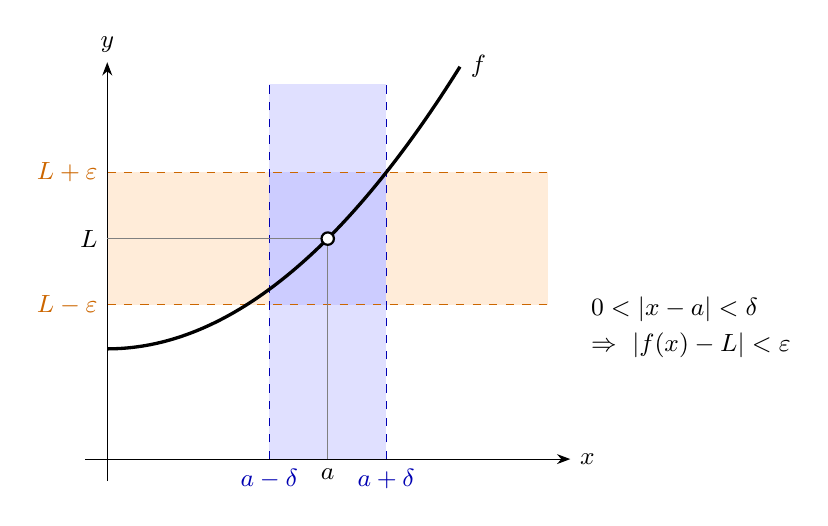
\begin{tikzpicture}[>={Stealth}, scale=1.4, every node/.style={font=\small}]
  % f(x) = x²/4 + 1, a = 2, L = 2, ε = 0.6; f(x) = 1.4 at x ≈ 1.265 and f(x) = 2.6 at x ≈ 2.530, so δ = 0.53 keeps x on both sides inside
  \fill[orange!15] (0,1.4) rectangle (4,2.6);
  \fill[blue!12] (1.47,0) rectangle (2.53,3.4);
  \fill[blue!25, opacity=0.6] (1.47,1.4) rectangle (2.53,2.6);
  \draw[dashed, orange!80!black] (0,1.4) node[left] {$L - \varepsilon$} -- (4,1.4) (0,2.6) node[left] {$L + \varepsilon$} -- (4,2.6);
  \draw[dashed, blue!70!black] (1.47,0) node[below] {$a - \delta$} -- (1.47,3.4) (2.53,0) node[below] {$a + \delta$} -- (2.53,3.4);
  \draw[->] (-0.2,0) -- (4.2,0) node[right] {$x$};
  \draw[->] (0,-0.2) -- (0,3.6) node[above] {$y$};
  \draw[very thick, black, domain=0:3.2, samples=60, smooth] plot (\x, {\x*\x/4 + 1}) node[right] {$f$};
  \draw[gray] (2,0) node[below, black] {$a$} -- (2,2) -- (0,2) node[left, black] {$L$};
  \fill[white, draw=black, thick] (2,2) circle (1.6pt);
  \node[align=left, anchor=west] at (4.3,1.2) {$0 < |x - a| < \delta$\\[2pt] $\Rightarrow\ |f(x) - L| < \varepsilon$};
\end{tikzpicture}
